\chapter{Evaluation}

\section{Technical Evaluation}
%Voxelizer, polygonization, queries, precision vs. recall?, etc.

This section is concerned with the technical performance of our application. These results should provide insight
into how the application performs to related work and reveal potential problems that may need to be improved on
in future work.

\subsection{ClusterD2+Color Performance}

\begin{figure}
\centering
\captionsetup{width=0.8\textwidth}
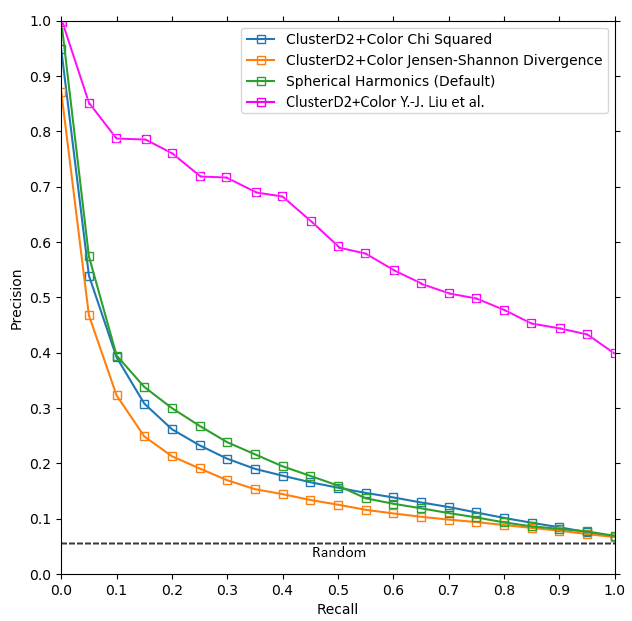
\includegraphics[width=0.5\textwidth]{precision_recall_chisqr_jsd_sh_liu.png}
\caption{Precision/recall plots comparing the performance of Y.-J. Liu et al.'s (pink) and our implementation (blue, orange) of the ClusterD2+Color algorithm using the McGill 3D shape benchmark and Cineast's "Spherical Harmonics (Default)" feature module (green). The random scoring baseline is calculated as the average of $\frac{P}{P+N}$ over all classes where $P$ is the number of positives and $N$ the number of negatives.}
\label{fig:precision_recall}
\end{figure}
\todoMissing{Missing ref; McGill 3D shape benchmark}

There are several ways to compare the performance and retrieval quality of different algorithms. One way to do so are precision/recall plots as shown in Fig. \ref{fig:precision_recall}. The larger the area under the
curve the better the algorithm performs. Our precision/recall plots have been computed in the same way as described by Y.-J. Liu et al. \todoMissing{Missing ref} and also using the same model benchmark dataset.\\
As can be seen in Fig. \ref{fig:precision_recall} our implementation of the ClusterD2+Color algorithm with both the Jensen-Shannon divergence distance metric, which Y.-J. Liu et al. used,
and the $\chi^2$ distance metric perform significantly worse than that of the original authors of the algorithm. This begs the question whether our implementation is faulty. Visual inspection, using our feature
extraction visualization tool, however shows no obvious errors. Both the shape and color feature samples are concentrated where one would expect and the cluster assignments also look sensible. The code that generates
the histogram feature vector from the clustered samples is simple and short so we deem it unlikely that it contains any errors.\\
One possible explanation could be the many parameters of the algorithm that can be tweaked. Several of these parameters were not specified by Y.-J. Liu et al. and thus had to be chosen and adjusted by us empirically
and may not be optimal.\\
On the other hand our ClusterD2+Color implementation performs similarly to Cineast's "Spherical Harmonics (Default)" feature module, whereas Y.-J. Liu et al.'s is suprisingly vastly better.
So perhaps the discrepancy between our and Y.-J. Liu et al.'s results could be caused by a difference in the McGill 3D shape benchmark [\todoMissing{Missing ref}] model dataset or in the way the precision/recall plots are computed. Finally, there's also the possibility that the result in [\todoMissing{Missing ref}] is incorrect.

\todoMissing{Query time?}

\subsection{Voxel Polygonizer Performance}
Time for an average chunk? Chunk size vs. time?

\subsection{Voxelizer Performance}
Before vs. after optimization. Plot tri count vs. time taken.

\section{User Evaluation}

\subsection{Structure}

\subsection{Results}

TBD after evaluation